\documentclass[a4paper,11pt]{exam}
\printanswers % pour imprimer les réponses (corrigé)
%\noprintanswers % Pour ne pas imprimer les réponses (énoncé)
\addpoints % Pour compter les points
% \noaddpoints % pour ne pas compter les points
\qformat{\textbf{\thequestion ) } }
\qformat{\textbf{\thequestion )} \textit{(\thepoints)} \\  } % Pour définir le style des questions (facultatif)
\usepackage{color} % définit une nouvelle couleur
\shadedsolutions % définit le style des réponses
% \framedsolutions % définit le style des réponses
\definecolor{SolutionColor}{rgb}{0.8,0.9,1} % bleu ciel
\renewcommand{\solutiontitle}{\noindent\textbf{Solution:}\par\noindent} % Définit le titre des solutions




\makeatletter

\def\maketitle{{\centering%
	\par{\huge\textbf{\@title}}%
	\par{\@date}%
	\par}}

\makeatother

\lhead{NOM Pr\'enom :}
\rhead{\textbf{Les r\'eponses doivent \^etre justifi\'ees}}
\cfoot{\thepage / \pageref{LastPage}}


%\usepackage{../../pas-math}
%\usepackage{../../moncours}


%\usepackage{pas-cours}
%-------------------------------------------------------------------------------
%          -Packages nécessaires pour écrire en Français et en UTF8-
%-------------------------------------------------------------------------------
\usepackage[utf8]{inputenc}
\usepackage[frenchb]{babel}
\usepackage[T1]{fontenc}
\usepackage{lmodern}
\usepackage{textcomp}



%-------------------------------------------------------------------------------

%-------------------------------------------------------------------------------
%                          -Outils de mise en forme-
%-------------------------------------------------------------------------------
\usepackage{hyperref}
\hypersetup{pdfstartview=XYZ}
%\usepackage{enumerate}
\usepackage{graphicx}
\usepackage{multicol}
\usepackage{tabularx}
\usepackage{multirow}


\usepackage{anysize} %%pour pouvoir mettre les marges qu'on veut
%\marginsize{2.5cm}{2.5cm}{2.5cm}{2.5cm}

\usepackage{indentfirst} %%pour que les premier paragraphes soient aussi indentés
\usepackage{verbatim}
\usepackage{enumitem}
\usepackage[usenames,dvipsnames,svgnames,table]{xcolor}

\usepackage{variations}

%-------------------------------------------------------------------------------


%-------------------------------------------------------------------------------
%                  -Nécessaires pour écrire des mathématiques-
%-------------------------------------------------------------------------------
\usepackage{amsfonts}
\usepackage{amssymb}
\usepackage{amsmath}
\usepackage{amsthm}
\usepackage{tikz}
\usepackage{xlop}
%-------------------------------------------------------------------------------



%-------------------------------------------------------------------------------


%-------------------------------------------------------------------------------
%                    - Mise en forme avancée
%-------------------------------------------------------------------------------

\usepackage{ifthen}
\usepackage{ifmtarg}


\newcommand{\ifTrue}[2]{\ifthenelse{\equal{#1}{true}}{#2}{$\qquad \qquad$}}

%-------------------------------------------------------------------------------

%-------------------------------------------------------------------------------
%                     -Mise en forme d'exercices-
%-------------------------------------------------------------------------------
%\newtheoremstyle{exostyle}
%{\topsep}% espace avant
%{\topsep}% espace apres
%{}% Police utilisee par le style de thm
%{}% Indentation (vide = aucune, \parindent = indentation paragraphe)
%{\bfseries}% Police du titre de thm
%{.}% Signe de ponctuation apres le titre du thm
%{ }% Espace apres le titre du thm (\newline = linebreak)
%{\thmname{#1}\thmnumber{ #2}\thmnote{. \normalfont{\textit{#3}}}}% composants du titre du thm : \thmname = nom du thm, \thmnumber = numéro du thm, \thmnote = sous-titre du thm

%\theoremstyle{exostyle}
%\newtheorem{exercice}{Exercice}
%
%\newenvironment{questions}{
%\begin{enumerate}[\hspace{12pt}\bfseries\itshape a.]}{\end{enumerate}
%} %mettre un 1 à la place du a si on veut des numéros au lieu de lettres pour les questions 
%-------------------------------------------------------------------------------

%-------------------------------------------------------------------------------
%                    - Mise en forme de tableaux -
%-------------------------------------------------------------------------------

\renewcommand{\arraystretch}{1.7}

\setlength{\tabcolsep}{1.2cm}

%-------------------------------------------------------------------------------



%-------------------------------------------------------------------------------
%                    - Racourcis d'écriture -
%-------------------------------------------------------------------------------

% Angles orientés (couples de vecteurs)
\newcommand{\aopp}[2]{(\vec{#1}, \vec{#2})} %Les deuc vecteurs sont positifs
\newcommand{\aopn}[2]{(\vec{#1}, -\vec{#2})} %Le second vecteur est négatif
\newcommand{\aonp}[2]{(-\vec{#1}, \vec{#2})} %Le premier vecteur est négatif
\newcommand{\aonn}[2]{(-\vec{#1}, -\vec{#2})} %Les deux vecteurs sont négatifs

%Ensembles mathématiques
\newcommand{\naturels}{\mathbb{N}} %Nombres naturels
\newcommand{\relatifs}{\mathbb{Z}} %Nombres relatifs
\newcommand{\rationnels}{\mathbb{Q}} %Nombres rationnels
\newcommand{\reels}{\mathbb{R}} %Nombres réels
\newcommand{\complexes}{\mathbb{C}} %Nombres complexes


%Intégration des parenthèses aux cosinus
\newcommand{\cosP}[1]{\cos\left(#1\right)}
\newcommand{\sinP}[1]{\sin\left(#1\right)}


%Probas stats
\newcommand{\stat}{statistique}
\newcommand{\stats}{statistiques}
%-------------------------------------------------------------------------------

%-------------------------------------------------------------------------------
%                    - Mise en page -
%-------------------------------------------------------------------------------

\newcommand{\twoCol}[1]{\begin{multicols}{2}#1\end{multicols}}


\setenumerate[1]{font=\bfseries,label=\textit{\alph*})}
\setenumerate[2]{font=\bfseries,label=\arabic*)}


%-------------------------------------------------------------------------------
%                    - Elements cours -
%-------------------------------------------------------------------------------




\usepackage{tabu}

%\usepackage{fullpage}
\author{\ }
\date{14 Février 2019}
\title{$T^{le}$ $ST_2S$ : DS num\'ero 3}


\begin{document}
%	\usepackage{fancyhdr}
%	
%	\pagestyle{fancy}
%	\fancyhf{}
	%\rhead{Share\LaTeX}

	\maketitle





%\section{Salariés d'une entreprise pharmaceutique}

Le tableau suivant donne la répartition des \num{1300} salariés d'une entreprise du secteur pharmaceutique en fonction de leur salaire moyen (exprimé en euros) et de leur sexe.

\begin{center}
	\begin{tabular}{|c|c|c|}
		\hline
		& Hommes & Femmes \\ \hline
		{[}1000 ; 1500{[}  & 440    & 400    \\ \hline
		{[}1500 ; 2000{[}  & 200    & 180    \\ \hline
		{[}2000  ; 2500{[} & 50     & 15     \\ \hline
		{[}2500 ; 3000{[}  & 10     & 5      \\ \hline
	\end{tabular}
\end{center}

\emph{Dans cet exercice, tous les résultats seront arrondis à $10^{-2} $. Dans chaque classe, on admet que la populations est au centre.}


\begin{questions}
	\question[3]\label{q:1} Déterminer :
		\begin{parts}
			\part[1] le salaire moyen de hommes ;
			\part[1] le salaire moyen des femmes ;
			\part[1] le salaire moyen de l'ensemble des salariés de l'entreprise.
		\end{parts} 
	
	\question[3] On note : 
	$H$ la sous population des hommes parmi les salariés, et $C$ la sous-population des cadres (les salariés ayant un salaire compris entre \num{2000} et \num{2500} euros).
	
	\begin{parts}
		\part[1] Calculer les fréquences respectives des, notées $f(H)$, $f(C)$, $f(H \cap C)$, des sous-populations $H$, $C$ et $H \cap C$ dans l'ensemble des salariés de l'entreprise.
		
		\part[1] \`A l'aide du tableau et des résultats obtenus au \ref{q:1} calculer la fréquence de la sous-population des cadres dans la sous-population des hommes. Cette fréquence appelée <<fréquence de $C$ sachant $H$>> est notée $f_H(C)$.
		
		\part[1] vérifier que $f_H(C) = \dfrac{f(H \cap C)}{f(H)}$
	\end{parts}
\end{questions}

%\newpage 

%\section{Taux d'évolution, ajustement affine}

Le tableau suivant donne la consommation de soins et biens médicaux (CSBM) en France de 2001 à 2008.

\begin{questions}
	\question[] Calculer le taux d'évolution de la CSBM entre 2001 et 2008. Arrondir à \num{0.01} \%.
	
	\question[] Calculer le montant des dépenses de médicaments en 2008 sachant qu'elles représentaient \num{24.47}  \% de la CSBM. Arrondir au milliard.
	
	\question[] Représenter par un nuage de points $M_i(x_i, y_i)$ la série statistique correspondant aux données du tableau. ON utilisera un repère orthogonal du plan tel que :
	\begin{itemize}
		\item 2 cm représentent une année sur l'axe des abscisses,
		
		\item 2 cm représentent 10 milliards d'euros sur l'axe des ordonnées (cet axe sera gradué de 100 à 200).
		
	\end{itemize}

	\question[] 
		\begin{parts}
			\part[] Calculer les coordonnées du point moyen G du nuage. Placer le point G sur le graphique.
			
			\part[] Soit $\delta$ la droite de coefficient directeur \num{6.7} passant par le point G ; déterminer une équation de la droite $\delta$. Tracer la droite $\delta$ sur le graphique.
			
			\part[] Cette droite vous paraît-elle représenter un bon ajustement du nuage de points ? Pourquoi ?
		\end{parts}
	
		\question[] On admet que l'ajustement réalisé par la droite $\delta$ est valable jusqu'en 2010. Déterminer graphiquement :
			\begin{parts}
				\part[]  Une estimation de la CSBM en 2010.
				\part[] l'année au cours de laquelle la CSBM a dépassé 175 milliards d'euros.
			\end{parts}
		
		\question[] justifier par le calcul les résultats de la question précédente.
\end{questions}

%\newpage 


\section{Boissons rafraichissantes (13 points)}

M. Ka vend des boissons rafraichissantes. Il note, six jours de suite, la température maximale de la journée et les ventes réalisées au cours de la journée.
Les résultats sont donnés dans le tableau suivant :

\vspace*{0.5cm}
\begin{center}
	
\begin{tabular}{|@{\ }l@{\ }|@{\ }c@{\ }|@{\ }c@{\ }|@{\ }c@{\ }|@{\ }c@{\ }|@{\ }c@{\ }|@{\ }c@{\ }|}
	\hline
	Jour                              & $1^{er}$ & $2^e$ & $3^e$ & $4^e$ & $5^e$ & $6^e$ \\ \hline
	Température (en °C), $x_i$        & 18       & 20    & 22    & 26    & 28    & 30    \\ \hline
	Nombre de boissons vendues, $y_i$ & 24       & 44    & 62    & 100   & 132   & 148   \\ \hline
\end{tabular}

\end{center}

\begin{questions}
	\question 
		\begin{parts}
			\part[2] Représenter le nuage de points de la série statistique (Axes orthogonaux ; unités : 1 cm pour 1°C en abscisse, en commençant à l'abscisse 17 ; 1 cm pour 10 boissons en ordonnée).
			
			\part[1] Indiquer pourquoi un ajustement affine est envisageable.
			\begin{solution}
				Un ajustement affine est envisageable car le nuage de point est allongé.
			\end{solution}
		\end{parts}
	
	\question[2] La droite $\Delta$ passe par les points du nuage de coordonnées $(20\; ; \;44)$ et $(30\; ; \;148)$, correspondant aux $2^e$ et $6^e$ jours. Donner son équation, et la tracer sur le graphique.
	\begin{solution}
		La droite $\Delta$ passe par les points $A(20\; ; \;44)$ et $B(30\; ; \;148)$.
		
		Calcul du coefficient directeur de la droite :
		
		\begin{eqnarray*}
			a &=& \frac{Y_B - Y_A}{X_B-X_A} \\
			a &=& \frac{148 - 44}{30 - 20} \\
			a &=& \frac{104}{10} \\
			a &=& \num{10.4}
		\end{eqnarray*}
		
		Donc la droite $\Delta$ a pour équation $y= \num{10.4} x + b$, calcul de l'ordonnée à l'origine, je remplace $x$ et $y$ par les coordonnées du point A :
		
		\begin{eqnarray*}
			y &=& \num{10.4} x + b \\
			44 &=& \num{10.4} \times 20 + b \\
			44 &=& 208 + b \\
			44 - 208 &=& b \\
			-164 &=& b
 		\end{eqnarray*}
 	
 		L'équation de la droite $\Delta$ est $y=\num{10.4} x - 164$.
	\end{solution}
	
	
	\question On choisit la droite d'équation  comme droite d'ajustement du nuage de points. 
	
	Estimer par le calcul en utilisant l'équation de cette droite :
	
		\begin{parts}
			\part[1\half] le nombre de boissons vendues pour une température de supérieure de 5°C à celle du $6^e$ jour;
			\begin{solution}
				Le $6^e$ jour la température était de 30°C, je recherche le nombre de boissons vendues pour une température de 35°C :
				
				\begin{eqnarray*}
					y &=& \num{10.4} x - 164 \\
					y &=& \num{10.4} \times 35 - 164\\
					y &=& 364 - 164 \\
					y &=& 200
				\end{eqnarray*}
			
				Pour une température de 35°C, il vendrait 200 boissons.
			\end{solution}
			
			\part[1] le nombre de boissons que vendrait  M. Ka pour une température de 25 °C;
			
			\begin{solution}
				Je recherche le nombre de boissons vendues pour une température de 25°C :
				
				\begin{eqnarray*}
					y &=& \num{10.4} x - 164 \\
					y &=& \num{10.4} \times 25 - 164\\
					y &=& 260 - 164 \\
					y &=& 96
				\end{eqnarray*}
				
				Pour une température de 25°C, il vendrait 96 boissons.
			\end{solution}
			
			\part[1\half] à partir de quelle température M. Ka vendrait au moins 160 boissons.
			
			\begin{solution}
				Je recherche la température correspondant à la vente de 160 boissons :
				
				\begin{eqnarray*}
					y &=& \num{10.4} x - 164 \\
					160 &=& \num{10.4} x - 164\\
					160 + 164 &=& \num{10.4} x \\
					324 &=& \num{10.4} x \\
					\frac{324}{\num{10.4}} &=& x \\
					31 &\approx& x 
				\end{eqnarray*}
				
				Pour une température d'environ 31°C, il vendrait 160 boissons.
			\end{solution}
		\end{parts}
	
	\question[2] Contrôler graphiquement les résultats de la question précédente en faisant apparaitre les tracés utiles.
	
	\question En fait, le $7^e$ jour, la température a augmenté de $20 \%$ par rapport au $6^e$ jour.
		\begin{parts}
			\part[1] Calculer la température du $7^e$ jour.
			\begin{solution}
				Le coefficient multiplicateur correspondant à une hausse de 20 \% est \num{1.2}.  Donc la température le  $7^e$ jour est de 36°C ($30 \times \num{1.2} = 36$).
			\end{solution}
			
			\part[1] En déduire une estimation du nombre de boissons vendues le $7^e$ jour à l'aide de l'équation de la droite d'ajustement.
			\begin{solution}
				Je recherche le nombre de boissons vendues pour une température de 36°C :
				
				\begin{eqnarray*}
					y &=& \num{10.4} x - 164 \\
					y &=& \num{10.4} \times 36 - 164\\
					y &=& \num{374.4} - 164 \\
					y &=& \num{210.4}
				\end{eqnarray*}
				
				Pour une température de 36°C, il vendrait 210 boissons.
			\end{solution}
		\end{parts}
		
\end{questions}

\newpage

\section{Une épidémie (7 points)}

Une épidémie affecte une île du Pacifique, depuis le mois d'avril 2013. Nous disposons des données du nombre de personnes infectées sur les mois d'avril à septembre 2013. Ces données sont récapitulées dans le tableau suivant :

\vspace*{0.5cm} 
\begin{center}
	\begin{tabular}{|@{\ }l@{\ }|@{\ }c@{\ }|@{\ }c@{\ }|@{\ }c@{\ }|@{\ }c@{\ }|@{\ }c@{\ }|@{\ }c@{\ }|}
		\hline
		Mois                                & Avril      & Mai        & Juin & Juillet    & Août & Septembre \\ \hline
		Rang du mois $x_i$                  & 0          & 1          & 2    & 3          & 4    & 5         \\ \hline
		Nombre de malades en milliers $y_i$ & \num{17.5} & \num{27.5} & 35   & \num{42.5} & 49   & 51        \\ \hline
	\end{tabular}
\end{center}

\begin{questions}
	\question[1] En observant le nuage de points correspondant au tableau, tracé ci-dessous, un ajustement affine est-il envisageable ?
	\begin{solution}
		Oui, un ajustement affine est envisageable car le nuage de point est allongé.
	\end{solution}
	
	\question[1\half] Calculer les coordonnées du point moyen $G$ du nuage de points et l'ajouter sur le nuage de points.
	\begin{solution}
		Calcul des coordonnées du point moyen G :
		
		\begin{eqnarray*}
			\bar{X} &=& \frac{0 + 1 + 2 + 3 + 4 + 5 }{6}\\
			\bar{X} &=& \frac{14}{6}\\
			\bar{X} &=& \num{2.5}
		\end{eqnarray*}
	
		\begin{eqnarray*}
			\bar{Y} &=& \frac{\num{17.5} + \num{27.5} + 35 + \num{42.5} + 49 + 51 }{6}\\
			\bar{Y} &=& \frac{\num{222.5}}{6}\\
			\bar{Y} &\approx& 37			
		\end{eqnarray*}
	
		Donc les coordonnées du point G sont $(\num{2.5}; 37)$.
	\end{solution}
	
	\question[2] On considère la droite $(d)$, d'équation $y = \num{6.8} x + 20$, réalise un bon ajustement du nuage de points. Tracer la droite $(d)$.
	
	\question En utilisant l'approximation affine précédente, déterminer par le calcul :
	\begin{parts}
		\part[1\half] le nombre de personnes atteintes en février 2014 ;
		
		\begin{solution}
			Le mois 0 est avril 2013, il y a 10 mois entre avril 2013 et février 2014. Je cherche le nombre de malades pour le mois de rang 10  :
			
			\begin{eqnarray*}
				y &=& \num{6.8} x + 20 \\
				y &=& \num{6.8} \times 10 - 20\\
				y &=& 68 + 20 \\
				y &=& 88
			\end{eqnarray*}
			
			En février 2014 il y aura \num{88000} personnes atteintes.
		\end{solution}
		\part[1\half] le mois à partir duquel la population atteinte dépassera \num{10000} personnes.
		\begin{solution}
			Je cherche le rang du mois où on dépassera les  \num{10000} malades :
			
			\begin{eqnarray*}
				y &=& \num{6.8} x + 20 \\
				100 &\leq& \num{6.8} \times x + 20\\
				100 - 20 &\leq& \num{6.8} \times x \\
				80 &\leq& \num{6.8} \times x \\
				\frac{80}{\num{6.8}} &\leq& x \\
				\num{11.7} &\leq& x
			\end{eqnarray*}
			
			Il faudra attendre plus de 11 mois pour dépasser les \num{100000} personnes atteintes, soit avril 2014.
		\end{solution}
	\end{parts}
	
\end{questions}

\begin{center}
	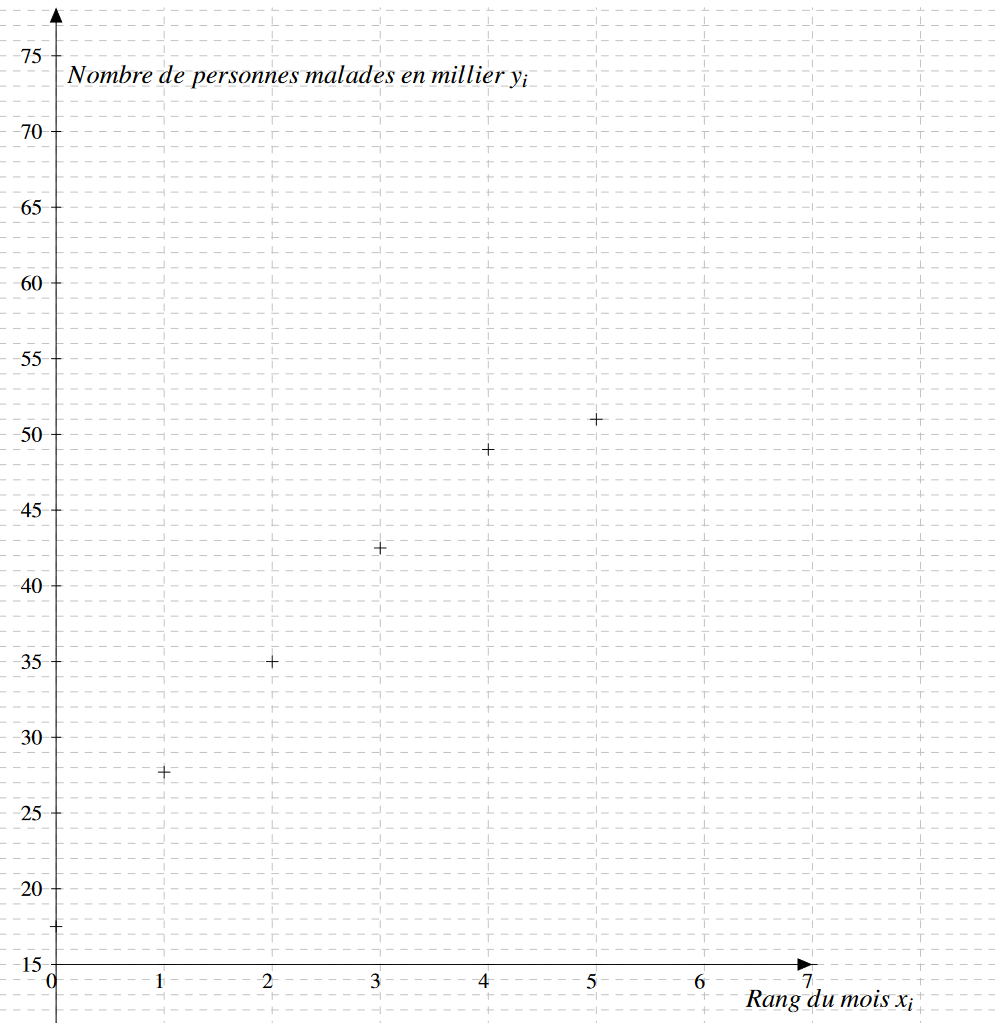
\includegraphics[scale=0.5]{nuage}
\end{center}

%\section{Un vrai-faux (6 points)}

Répondez par VRAI ou FAUX aux affirmations suivantes. Une justification est demandée lorsque la réponse est FAUX, aucune justification n'est demandée lorsque la réponse est VRAI.

\begin{questions}
	\question[1] Pour une série ordonnée comptant 512 nombres, la médiane n'existe pas car 512 est pair.
	
	\question[1] En France, le salaire mensuel moyen s'élève à \num{2500} € et le salaire mensuel médian s'élève à \num{1600} €. Plus de 50 \% des salariés gagnent moins de \num{2500} € par mois.
	
	\question[1] Le couple médiane et écart interquartile est peu sensible aux valeurs extrêmes de la série statistique.
	
	\question[1] La moyenne rend compte de la dispersion de la série statistique.
	
	\question[1] Si une série statistique compte 10 valeurs, les quartiles sont toujours des valeurs de la série.
	
	\question[1] On donne la série : 1 ; 2 ; 3 ; 4 ; 4 ; 4 ; 5 ; 8 ; 9 ; 10. L'écart interquartille est 5.
\end{questions}

\label{LastPage}
	

\end{document}